% Options for packages loaded elsewhere
\PassOptionsToPackage{unicode}{hyperref}
\PassOptionsToPackage{hyphens}{url}
\PassOptionsToPackage{dvipsnames,svgnames,x11names}{xcolor}
%
\documentclass[
  a4paper,
]{scrreport}

\usepackage{amsmath,amssymb}
\usepackage{iftex}
\ifPDFTeX
  \usepackage[T1]{fontenc}
  \usepackage[utf8]{inputenc}
  \usepackage{textcomp} % provide euro and other symbols
\else % if luatex or xetex
  \usepackage{unicode-math}
  \defaultfontfeatures{Scale=MatchLowercase}
  \defaultfontfeatures[\rmfamily]{Ligatures=TeX,Scale=1}
\fi
\usepackage{lmodern}
\ifPDFTeX\else  
    % xetex/luatex font selection
\fi
% Use upquote if available, for straight quotes in verbatim environments
\IfFileExists{upquote.sty}{\usepackage{upquote}}{}
\IfFileExists{microtype.sty}{% use microtype if available
  \usepackage[]{microtype}
  \UseMicrotypeSet[protrusion]{basicmath} % disable protrusion for tt fonts
}{}
\makeatletter
\@ifundefined{KOMAClassName}{% if non-KOMA class
  \IfFileExists{parskip.sty}{%
    \usepackage{parskip}
  }{% else
    \setlength{\parindent}{0pt}
    \setlength{\parskip}{6pt plus 2pt minus 1pt}}
}{% if KOMA class
  \KOMAoptions{parskip=half}}
\makeatother
\usepackage{xcolor}
\setlength{\emergencystretch}{3em} % prevent overfull lines
\setcounter{secnumdepth}{5}
% Make \paragraph and \subparagraph free-standing
\ifx\paragraph\undefined\else
  \let\oldparagraph\paragraph
  \renewcommand{\paragraph}[1]{\oldparagraph{#1}\mbox{}}
\fi
\ifx\subparagraph\undefined\else
  \let\oldsubparagraph\subparagraph
  \renewcommand{\subparagraph}[1]{\oldsubparagraph{#1}\mbox{}}
\fi


\providecommand{\tightlist}{%
  \setlength{\itemsep}{0pt}\setlength{\parskip}{0pt}}\usepackage{longtable,booktabs,array}
\usepackage{calc} % for calculating minipage widths
% Correct order of tables after \paragraph or \subparagraph
\usepackage{etoolbox}
\makeatletter
\patchcmd\longtable{\par}{\if@noskipsec\mbox{}\fi\par}{}{}
\makeatother
% Allow footnotes in longtable head/foot
\IfFileExists{footnotehyper.sty}{\usepackage{footnotehyper}}{\usepackage{footnote}}
\makesavenoteenv{longtable}
\usepackage{graphicx}
\makeatletter
\def\maxwidth{\ifdim\Gin@nat@width>\linewidth\linewidth\else\Gin@nat@width\fi}
\def\maxheight{\ifdim\Gin@nat@height>\textheight\textheight\else\Gin@nat@height\fi}
\makeatother
% Scale images if necessary, so that they will not overflow the page
% margins by default, and it is still possible to overwrite the defaults
% using explicit options in \includegraphics[width, height, ...]{}
\setkeys{Gin}{width=\maxwidth,height=\maxheight,keepaspectratio}
% Set default figure placement to htbp
\makeatletter
\def\fps@figure{htbp}
\makeatother

%\newfontfamily\Ubuntu[Mapping=tex-text]{Ubuntu}
\usepackage{pgfplots}
\usetikzlibrary{arrows.meta,arrows}
\usetikzlibrary{angles,quotes}
\pgfplotsset{grid style={dashed,mygray}}
% Colors
\definecolor{myblue}{rgb}{0.067,0.529,0.871}
\definecolor{mypurple}{rgb}{0.859,0.071,0.525}
\definecolor{myred}{rgb}{1.0, 0.13, 0.32}
\definecolor{mygreen}{rgb}{0.01, 0.75, 0.24}
\definecolor{myblack}{gray}{0.1}
\definecolor{mygray}{gray}{0.8}
\newcommand{\NN}{\mathbb{N}}
\newcommand{\ZZ}{\mathbb{Z}}
\newcommand{\QQ}{\mathbb{Q}}
\newcommand{\RR}{\mathbb{R}}
\newcommand{\CC}{\mathbb{C}}
\DeclareMathOperator{\operatorname{Int}}{Int}
\DeclareMathOperator{\operatorname{Ext}}{Ext}
\DeclareMathOperator{\operatorname{Fr}}{Fr}
\DeclareMathOperator{\Adh}{Adh}
\DeclareMathOperator{\Ac}{Ac}
\DeclareMathOperator{\sen}{sen}
\makeatletter
\makeatother
\makeatletter
\@ifpackageloaded{bookmark}{}{\usepackage{bookmark}}
\makeatother
\makeatletter
\@ifpackageloaded{caption}{}{\usepackage{caption}}
\AtBeginDocument{%
\ifdefined\contentsname
  \renewcommand*\contentsname{Tabla de contenidos}
\else
  \newcommand\contentsname{Tabla de contenidos}
\fi
\ifdefined\listfigurename
  \renewcommand*\listfigurename{Listado de Figuras}
\else
  \newcommand\listfigurename{Listado de Figuras}
\fi
\ifdefined\listtablename
  \renewcommand*\listtablename{Listado de Tablas}
\else
  \newcommand\listtablename{Listado de Tablas}
\fi
\ifdefined\figurename
  \renewcommand*\figurename{Figura}
\else
  \newcommand\figurename{Figura}
\fi
\ifdefined\tablename
  \renewcommand*\tablename{Tabla}
\else
  \newcommand\tablename{Tabla}
\fi
}
\@ifpackageloaded{float}{}{\usepackage{float}}
\floatstyle{ruled}
\@ifundefined{c@chapter}{\newfloat{codelisting}{h}{lop}}{\newfloat{codelisting}{h}{lop}[chapter]}
\floatname{codelisting}{Listado}
\newcommand*\listoflistings{\listof{codelisting}{Listado de Listados}}
\usepackage{amsthm}
\theoremstyle{definition}
\newtheorem{exercise}{Ejercicio}[chapter]
\theoremstyle{remark}
\AtBeginDocument{\renewcommand*{\proofname}{Prueba}}
\newtheorem*{remark}{Observación}
\newtheorem*{solution}{Solución}
\makeatother
\makeatletter
\@ifpackageloaded{caption}{}{\usepackage{caption}}
\@ifpackageloaded{subcaption}{}{\usepackage{subcaption}}
\makeatother
\makeatletter
\@ifpackageloaded{tcolorbox}{}{\usepackage[skins,breakable]{tcolorbox}}
\makeatother
\makeatletter
\@ifundefined{shadecolor}{\definecolor{shadecolor}{rgb}{.97, .97, .97}}
\makeatother
\makeatletter
\makeatother
\makeatletter
\makeatother
\ifLuaTeX
\usepackage[bidi=basic]{babel}
\else
\usepackage[bidi=default]{babel}
\fi
\babelprovide[main,import]{spanish}
% get rid of language-specific shorthands (see #6817):
\let\LanguageShortHands\languageshorthands
\def\languageshorthands#1{}
\ifLuaTeX
  \usepackage{selnolig}  % disable illegal ligatures
\fi
\IfFileExists{bookmark.sty}{\usepackage{bookmark}}{\usepackage{hyperref}}
\IfFileExists{xurl.sty}{\usepackage{xurl}}{} % add URL line breaks if available
\urlstyle{same} % disable monospaced font for URLs
\hypersetup{
  pdftitle={Problemas de Análisis Matemático},
  pdfauthor={Alfredo Sánchez Alberca},
  pdflang={es},
  colorlinks=true,
  linkcolor={blue},
  filecolor={Maroon},
  citecolor={Blue},
  urlcolor={Blue},
  pdfcreator={LaTeX via pandoc}}

\title{Problemas de Análisis Matemático}
\author{Alfredo Sánchez Alberca}
\date{2022-01-06}

\begin{document}
\begin{titlepage}

%\AddToShipoutPicture*{\put(0,0){\includegraphics[scale=0.8]{img/background2}}} % Imagen de fondo, requiere el paquete eso-pic.
\begin{center}
\vspace*{5cm}

\Huge
{\textbf{\textsf{Problemas de Análisis Matemático}}}

\vspace{0.5cm}
\LARGE
{\textbf{\textsf{}}}

\vspace{1.5cm}

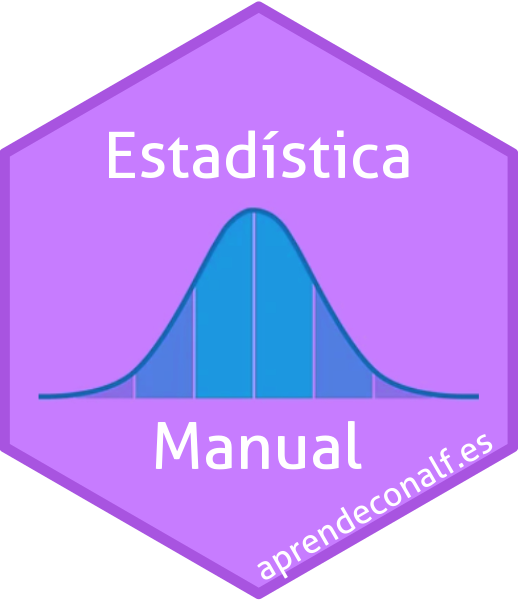
\includegraphics[width=0.4\textwidth]{img/logos/sticker.png}
\end{center}

\vfill

\begin{flushleft}
\begin{tabular}{ll}

\includegraphics[width=0.1\textwidth]{img/logos/aprendeconalf.png} & \parbox[b]{5cm}{\Large\textsf{Alfredo
Sánchez
Alberca}\\ \textsf{asalber@ceu.es} \\ \textsf{https://aprendeconalf.es}}
\end{tabular}
\end{flushleft}
\end{titlepage}\ifdefined\Shaded\renewenvironment{Shaded}{\begin{tcolorbox}[interior hidden, frame hidden, borderline west={3pt}{0pt}{shadecolor}, sharp corners, boxrule=0pt, breakable, enhanced]}{\end{tcolorbox}}\fi

\renewcommand*\contentsname{Tabla de contenidos}
{
\hypersetup{linkcolor=}
\setcounter{tocdepth}{2}
\tableofcontents
}
\bookmarksetup{startatroot}

\hypertarget{prefacio}{%
\chapter*{Prefacio}\label{prefacio}}
\addcontentsline{toc}{chapter}{Prefacio}

\markboth{Prefacio}{Prefacio}

Colección de problemas de Estadística aplicada a la Economía para el
Master en Análisis y Comunicación de Datos.

\bookmarksetup{startatroot}

\hypertarget{estimaciuxf3n-de-paruxe1metros}{%
\chapter{Estimación de
parámetros}\label{estimaciuxf3n-de-paruxe1metros}}

\begin{exercise}[]\protect\hypertarget{exr-distribucion-media-trabajadores-pymes}{}\label{exr-distribucion-media-trabajadores-pymes}

El número medio de trabajadores en las PYMES españolas es 5 y su
varianza 4. Realizado un muestreo aleatorio de 16 PYMES.

Calcular:

\begin{enumerate}
\def\labelenumi{\alph{enumi}.}
\item
  La esperanza y varianza de la media muestral.
\item
  La esperanza de la varianza y de la cuasivarianza muestral.
\item
  Mínimo tamaño que ha de tener la muestra para que exista una
  probabilidad mayor o igual al \(95\)\% de que la media muestral se
  desvíe de la media poblacional a lo sumo \(0.25\) unidades.
\item
  Si realizamos un muestreo aleatorio de tamaño \(320\) obtener
  \(P(4.9\leq \bar x \leq 5.2.\).
\end{enumerate}

\end{exercise}

\begin{exercise}[]\protect\hypertarget{exr-distribucion-cuasivarianza-iberpapel}{}\label{exr-distribucion-cuasivarianza-iberpapel}

El precio de las acciones de Iberpapel se distribuyen según un modelo
normal \(N(\mu, 2.\), analizar \(16\) sesiones de la Bolsa de Madrid
elegidas aleatoriamente, para calcular la probabilidad de que la
cuasivarianza muestral del precio de las acciones sea mayor o igual que
\(2.136\).

\end{exercise}

\begin{exercise}[]\protect\hypertarget{exr-diferencia-proporciones-votos}{}\label{exr-diferencia-proporciones-votos}

El porcentaje de votantes con preferencia de un determinado partido es
del \(5\)\% en una región \(A\), y el \(10\)\% en otra \(B\).
Consultados \(100\) electores de la región \(A\) y \(150\) de la \(B\),
determinar la probabilidad de que el porcentaje de electores consultados
favorables a dicho partido en la segunda región supere en más de
\(0.02\) al porcentaje de electores favorables a dicho partido en la
primera.

\end{exercise}

Una empresa desea estudiar la demanda futura de uno de sus productos,
para lo cual selecciona, mediante muestreo aleatorio simple, a diez de
sus clientes, observando el número de unidades demandadas por ellos:

\begin{longtable}[]{@{}rr@{}}
\toprule\noalign{}
Número de unidades demandadas & Número de clientes \\
\midrule\noalign{}
\endhead
\bottomrule\noalign{}
\endlastfoot
1000 & 1 \\
1002 & 2 \\
1004 & 1 \\
1006 & 2 \\
1008 & 1 \\
1010 & 2 \\
1012 & 1 \\
\end{longtable}

Suponiendo que la demanda sigue una distribución normal.

\begin{enumerate}
\def\labelenumi{\alph{enumi}.}
\tightlist
\item
  Estimar la demanda media mediante un intervalo de confianza con nivel
  de significación \(0.1\).
\item
  ¿Qué tamaño muestral sería necesario para que el intervalo tuviese un
  error máximo de \(\pm 2\) unidades?
\end{enumerate}

\begin{exercise}[]\protect\hypertarget{exr-intervalo-confianza-media-bitcoin}{}\label{exr-intervalo-confianza-media-bitcoin}

Al objeto de determinar la proporción de españoles que poseen la
criptomoneda bitcoin se ha realizado un muestreo aleatorio de \(100\)
españoles, resultando que \(15\) tienen bitcoins.

\begin{enumerate}
\def\labelenumi{\alph{enumi}.}
\item
  Obtener un intervalo de confianza del \(95\)\% para la proporción
  poblacional de españoles que poseen bitcoins.
\item
  ¿A cuántos españoles se debería encuestar para lograr una semiamplitud
  del intervalo de \(0.02\), utilizando un nivel de confianza del
  \(80\)\%?
\end{enumerate}

\end{exercise}

\begin{exercise}[]\protect\hypertarget{exr-intervalo-confianza-proporcion-demanda}{}\label{exr-intervalo-confianza-proporcion-demanda}

Una empresa quiere conocer la proporción de clientes dispuestos a
demandar un nuevo producto, para averiguarlo efectúa un muestreo
aleatorio de tamaño \(100\) en el que se obtiene que un \(20\)\% de
ellos estarían dispuestos a comprar el nuevo producto. Determinar el
intervalo de confianza para la proporción poblacional con un grado de
confianza del \(90\)\%.

\end{exercise}

\begin{exercise}[]\protect\hypertarget{exr-intervalo-confianza-media-varianza-gasto-alimentacion}{}\label{exr-intervalo-confianza-media-varianza-gasto-alimentacion}

En una comunidad autónoma, los gastos semanales en alimentación por
unidad familiar se distribuyen según un modelo normal \(N(\mu,\sigma.\).
Realizado un muestreo aleatorio en el que se han consultado a \(21\)
unidades familiares hemos obtenido que el gasto medio semanal muestral
es de \(150\) euros y la cuasidesviación típica semanal muestral es de
\(12\) euros.

\begin{enumerate}
\def\labelenumi{\alph{enumi}.}
\item
  Construir un intervalo de confianza del \(95\)\% para el gasto medio
  semanal poblacional.
\item
  Construir un intervalo de confianza del \(95\)\% para la varianza
  poblacional.
\end{enumerate}

\end{exercise}

\begin{exercise}[]\protect\hypertarget{exr-intervalo-confianza-media-varianza-gasto-porcino}{}\label{exr-intervalo-confianza-media-varianza-gasto-porcino}

Los gastos mensuales en carne de porcino en las familias españolas se
distribuyen según un modelo normal \(N(\mu, \sigma.\). Realizando un
muestreo aleatorio en el que se pregunta a \(20\) unidades familiares,
se obtiene que el gasto medio mensual ha sido de \(170.31\) € y la
cuasidesviación típica de \(36\) €.

\begin{enumerate}
\def\labelenumi{\alph{enumi}.}
\item
  Obtener el intervalo de confianza para el gasto medio mensual en carne
  de porcino con un \(95\)\% de confianza.
\item
  Razone cómo podría obtener un intervalo de confianza más preciso para
  el gasto medio, suponiendo que no varían la media muestral, la
  cuasivarianza muestral y el tamaño de la muestra.
\item
  Obtener el intervalo de confianza para la varianza del gasto mensual
  en carne de porcino con un \(95\)\% de confianza.
\end{enumerate}

\end{exercise}

\begin{exercise}[]\protect\hypertarget{exr-intervalo-confianza-media-peso}{}\label{exr-intervalo-confianza-media-peso}

La OMS ha obtenido una muestra de los pesos de \(50\) niños de entre
\(11\) y \(14\) años, que proporciona una media muestral de \(47\) kg y
una desviación típica muestral de \(11\) kg. Suponiendo que la población
sigue una distribución normal.

\begin{enumerate}
\def\labelenumi{\alph{enumi}.}
\item
  Obtener un intervalo de confianza para la media poblacional con un
  \(95\)\% de nivel de confianza.
\item
  El director de la OMS considera que el intervalo es insatisfactorio,
  pero quiere mantener el nivel de confianza. Por ello decide reducir a
  la mitad la precisión de dicho intervalo (reducir un \(50\)\% el radio
  del intervalo.. En estas condiciones, ¿cuál debería ser el tamaño de
  la muestra para cumplir los objetivos del director?
\item
  Los resultados obtenidos en los análisis anteriores siguen sin
  convencer al director de la OMS y le pide a su equipo que establezca
  un intervalo de confianza para la media poblacional con un \(99\)\% de
  nivel de confianza, manteniendo la misma muestra del ejercicio
  anterior.
\item
  El director decide reducir en un tercio la precisión del intervalo
  anterior, pero quiere mantener el nivel de confianza ¿cuál debería ser
  el tamaño de la muestra para cumplir dicho objetivo?
\end{enumerate}

\end{exercise}

\begin{exercise}[]\protect\hypertarget{exr-intervalo-confianza-proporcion-uso-alta-velocidad}{}\label{exr-intervalo-confianza-proporcion-uso-alta-velocidad}

Tras la liberalización del transporte ferroviario de pasajeros en las
líneas de alta velocidad en España, la compañía francesa SNCF estudia la
proporción de clientes que utiliza al menos una vez al mes el servicio
de alta velocidad. A tal efecto la empresa realiza un muestreo aleatorio
en el que se seleccionan \(50\) usuarios y en el que resulta que \(35\)
de ellos afirma utilizar este servicio una vez al mes como mínimo.

Considerando un nivel de confianza del \(98\)\% determine un intervalo
de confianza poblacional para la proporción de usuarios que utilizan la
alta velocidad una vez al mes por lo menos (justifique cómo obtiene el
intervalo de confianza antes de proceder a su cálculo..

\end{exercise}



\end{document}
